\section{Modelli di secondo grado}


\subsection{Equazioni}
\begin{questions}


\question
\exonly{Risolvi le seguenti equazioni }

\begin{multicols}{2}
	\begin{parts}
		\setlength\itemsep{4mm}
		\part \exonly{$ 3x^2-5x=0 $	 }			
		\part \exonly{$ 3 x^2-5 =x^2+7$ }
		\part \exonly{$ 3(x^2-2)=5-x^2$ }
		\part \exonly{$ 2x(x-3)=(2-x)x $ }
		\part \exonly{$ 5x^2-3x-4=(x+2)(x-2) $ }
		\part \exonly{$ (x+3)(x+2)=2(x-3)(x-1)$ }
		\part \exonly{ $ 3x^2-5x=0 $ }
		\part \exonly{$ 2x^2+3x=0 $ }
		\part \exonly{ $ x^2-3x+2=-3(x-4) $ }
		\part \exonly{$ (2x+1)(x+2)=(1-x)(x-4) $ }
	\end{parts}
\end{multicols}


\question

\exonly{ Risolvi le seguenti equazioni: }
\begin{multicols}{2}
	\begin{parts}
		\setlength\itemsep{4mm}
		\part \exonly{ $ 2x^2-3x+5=0 $ }
		\part \exonly{$ 2x+1-3x^2=2x^2-5x+1 $ }
		\part \exonly{$ (x+3)(2x-5)=(3x+1)(2-x) $ }
		\part \exonly{$ \frac{2}{3}x^2+\frac{1}{4}x-\frac{1}{2}=0 $ }
		\part \exonly{ $ (\frac{1}{2}x+\frac{1}{3})(x-2)=\frac{2}{3}(x+\frac{1}{3})(x+\frac{2}{3}) $ }
		\part \exonly{$ \frac{2}{3}x^2-\frac{3}{2}x+\frac{1}{4}= \frac{1}{5}x^2-\frac{1}{3}x-\frac{2}{5} $ }
	\end{parts}
\end{multicols}

\end{questions}

\exnewpage
\subsection{Funzioni e rappresentazione grafica}

\begin{questions}	

\question
	
\exonly{
	Data la parabola di equazione:
	
	$$y=2x^ 2 -4x-11$$
}
	
	\begin{parts}
		\part
			\exonly{ Calcolare le coordinate del vertice }
			\solonly{$V(1,-13)$ }
			
		\part
			\exonly{Calcolare i punti di intersezione della parabola con l'asse delle ascisse. }
			\solonly{ $I_x=\{(3.55;0),(-1.55;0)\}$}
		\part
			\exonly{Calcolare i punti di intersezione della parabola con l'asse delle ordinate. }	
			\solonly{$I_y(0,-11)$ }
	\end{parts}


	
	\question
\exonly{	
	Calcolare le coordinate $x_A$ e $y_B$ tali per cui i punti $A(x_A;-5)$ e $B(-8;y_B)$ appartengano alla parabola di equazione 

	
	$$y= -\dfrac{1}{2}x^2-6x-\dfrac{21}{2}$$ }
\solonly{ 	$x_A=\{-11,-1\}$
	
	$y_B=\frac{11}{2}$}
	

	
	\question
	
	
\exonly{
	Calcolare i punti di intersezione tra la parabola di equazione
	
	$$y= \dfrac{1}{4}x^2+4x+6$$
	
	e la retta di equazione
	
	$$y= 2x +3$$ }
	
	\solonly{$	S=\{(-2;-1),(-6;-9)\}$}
	
	
%	\question
%	
%\exonly{	Calculez les points d'intersection de la parabole 
%	
%	$$y= \dfrac{1}{2}x^2+7x-3$$
%	
%	avec la parabole
%	
%	$$y= -\dfrac{5}{2}x^2+4x+3$$ }
%	
%	\rsol{	$S=\{(1;\frac{9}{2}),(-2;-15)\}$}
%	
\question

	\exonly{
	Determinare il parametro $b$ tale per cui la parabola di equazione $y=x^2+b \cdot x +4$  passi per il punto $A(4;4)$. }
	
\solonly{$b=-4$ , $y=x^2-4x+4$}

\question
\exonly{Determinare l’equazione di una parabola passante per i seguenti punti: $(2; 3)$, $(-1; 6)$ e $(4; 21)$. }
\solonly{$x=2x^2-3x+1$ }

\question

\exonly{

La somma di due numeri è $36$. Determinare questi due numeri sapendo che il loro
prodotto è massimo. }

\solonly{$18$ e $18$ }

%\exnewpage
\question
\exonly{
Un’azienda fabbrica un certo oggetto la cui domanda $x$ è data dalla funzione
$x = 10200 - 300p$ dove $p$ rappresenta il possibile prezzo di vendita  dell'oggetto.

I costi fissi ammontano a \SI{14400}{\CHF} e i costi variabili a \SI{8}{\CHF}  per oggetto prodotto. 
}

\begin{parts}
	\part
	\exonly{Determinare la funzione dei costi $C(p)$ in funzione del prezzo $p$.  }
	\solonly{$C(p)=-\num{2400}p+\num{96000}$ }
	\part
	\exonly{Determinare la funzione dei ricavi $R(p)$ in funzione del prezzo $p$.  }
	\solonly{$R(p)=-300p^2+\num{10200}$ }
	\part
	\exonly{Determinare la funzione del guadagno (beneficio) $G(p)$ in funzione del prezzo $p$.  }
	\solonly{$G(p)=-300p^2+\num{12600}p -\num{96000}$ }
	\part
	\exonly{ Determinare il prezzo $p$ che massimizzi il guadagno. Di seguito determinare il guadagno massimo.}
	\solonly{Prezzo che massimizza il guadagno \SI{21}{\CHF}. Guadagno massimo \SI{36300}{\CHF} }

	
\end{parts}



\question
\exonly{
	Rappresenta graficamente le seguenti funzioni. Trova le intersezioni con gli assi e le coordinate del vertice }

	\begin{multicols}{2}
		\begin{parts}
			\setlength\itemsep{4mm}
			\part 
			\exonly{$\begin{aligned}[t]
			f:\mathbb{R} & \longrightarrow\mathbb{R}\\
			x & \longmapsto 3x^2-5			
			\end{aligned}$ }
			\part 
		\exonly{	$
			\begin{aligned}[t]
			f:\mathbb{R} & \longrightarrow\mathbb{R}\\
			x & \longmapsto -\frac{1}{4}x^2-1	
			\end{aligned}$ }
			\part 
			\exonly{$
			\begin{aligned}[t]
			f:\mathbb{R} & \longrightarrow\mathbb{R}\\
			x & \longmapsto 2x^2+3x	
			\end{aligned}$ }
			\part
			\exonly{ $
			\begin{aligned}[t]
			f:\mathbb{R} & \longrightarrow\mathbb{R}\\
			x & \longmapsto -\frac{1}{2}x^2+5x	
			\end{aligned}$ }
			\part 
			\exonly{$
			\begin{aligned}[t]
			f:w\mathbb{R} & \longrightarrow\mathbb{R}\\
			x & \longmapsto x^2-4x-32	
			\end{aligned}$ }
			\part 
			\exonly{$
			\begin{aligned}[t]
			f:\mathbb{R} & \longrightarrow\mathbb{R}\\
			x & \longmapsto 2x^2-5x-3	
			\end{aligned}$ }
		\end{parts}
	\end{multicols}




\question

\exonly{	Sono date le seguenti funzioni: 
	\begin{multicols}{2}
		\begin{itemize}
			\setlength\itemsep{4mm}
			\item $
			\begin{aligned}[t]
			f:\mathbb{R} & \longrightarrow\mathbb{R}\\
			x & \longmapsto 2x^2+3x-5			
			\end{aligned}$
			\item $
			\begin{aligned}[t]
			g:\mathbb{R} & \longrightarrow\mathbb{R}\\
			x & \longmapsto -\frac{1}{4}x^2-\frac{3}{5}x+\frac{2}{3}
			\end{aligned}$
		\end{itemize}
	\end{multicols}
}
	\begin{parts}
		\part \exonly{Trova le intersezioni di $f$ e di $g$ con gli assi.  }
		\part \exonly{Trova le intersezioni di $f$ con $g$. }
		\part \exonly{Trova le coordinate dei due vertici. }
	\end{parts}


	
\question

\exonly{	Sono date le seguenti funzioni:

	\begin{multicols}{2}
		\begin{itemize}
			\setlength\itemsep{4mm}
			\item $
			\begin{aligned}[t]
			f:\mathbb{R} & \longrightarrow\mathbb{R}\\
			x & \longmapsto x^2+2x-4			
			\end{aligned}$
			\item $
			\begin{aligned}[t]
			g:\mathbb{R} & \longrightarrow\mathbb{R}\\
			x & \longmapsto -2x^2-3x+4
			\end{aligned}$
			\item $
			\begin{aligned}[t]
			h:\mathbb{R} & \longrightarrow\mathbb{R}\\
			x & \longmapsto -3x^2+x-2			
			\end{aligned}$
			\item $
			\begin{aligned}[t]
			i:\mathbb{R} & \longrightarrow\mathbb{R}\\
			x & \longmapsto \frac{1}{2}x^2-\frac{2}{3}x+\frac{5}{3}
			\end{aligned}$
		\end{itemize}
	\end{multicols}

		\begin{parts}
			\part Disegnare uno schizzo del grafico di ogni funzione senza calcolarne i punti.
			\part Disegnare il grafico esatto (calcolando i punti) e confrontalo con lo schizzo.
		\end{parts}
}

\exnewpage
\question

\exonly{ Determinare l'equazione delle funzioni di cui sono dati i grafici:
}
	\begin{multicols}{2}
	\begin{parts}
		
		\part
		\exonly{
		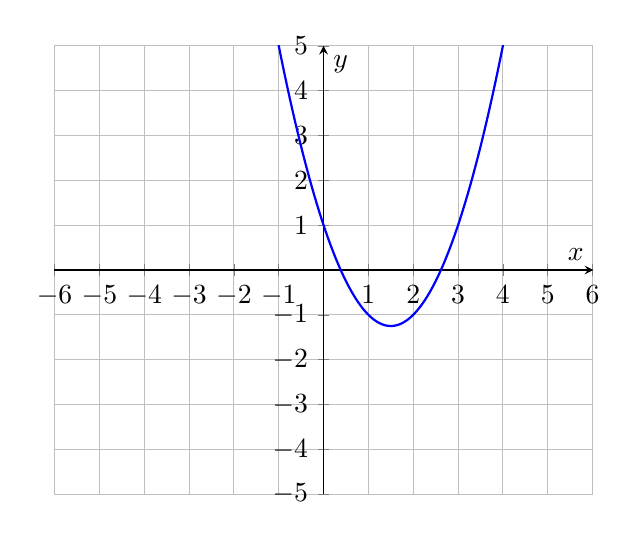
\begin{tikzpicture}
			\begin{axis}[
			axis equal,
			axis x line=middle, 
			axis y line=middle,
			xlabel={$x$},		
			ylabel={$y$},
			xtick={-6,-5,...,6}, 
			ytick={-5,-4,...,5},
%			minor tick num = 2,
			xmin=-4, xmax=4,
			ymin=-5, ymax=5,
			grid=both,]
			\addplot[domain=-6:6,			samples=200,thick,color=blue,]{x^2-3*x+1};	
			\end{axis}
		\end{tikzpicture}
		}
		\solonly{$y=x^2-3x+1$}
		
		\part
		\exonly{
			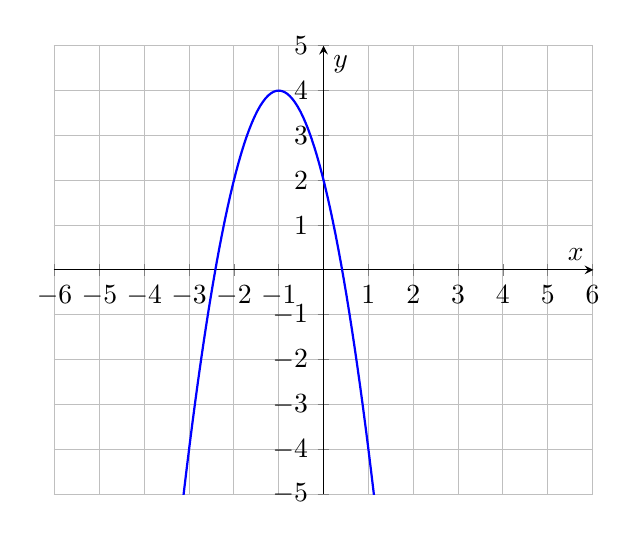
\begin{tikzpicture}
			\begin{axis}[
			axis equal,
			axis x line=middle, 
			axis y line=middle,
			xlabel={$x$},		
			ylabel={$y$},
			xtick={-6,-5,...,6}, 
			ytick={-5,-4,...,5},
			%			minor tick num = 2,
			xmin=-4, xmax=4,
			ymin=-5, ymax=5,
			grid=both,]
			\addplot[domain=-6:6,			samples=200,thick,color=blue,]{-2*x^2-4*x+2};	
			\end{axis}
			\end{tikzpicture}
		}
		\solonly{$y=-2x^2-4x+2$}
		
		\part
		\exonly{
			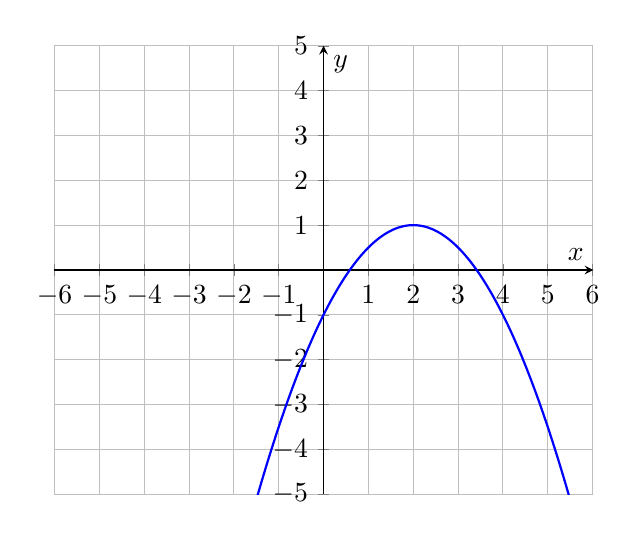
\begin{tikzpicture}
			\begin{axis}[
			axis equal,
			axis x line=middle, 
			axis y line=middle,
			xlabel={$x$},		
			ylabel={$y$},
			xtick={-6,-5,...,6}, 
			ytick={-5,-4,...,5},
			%			minor tick num = 2,
			xmin=-4, xmax=4,
			ymin=-5, ymax=5,
			grid=both,]
			\addplot[domain=-6:6,			samples=200,thick,color=blue,]{-1/2*x^2+2*x-1};	
			\end{axis}
			\end{tikzpicture}
		}
		\solonly{$y=-\frac{1}{2}x^2+2x-1$}
		
		\part
		\exonly{
			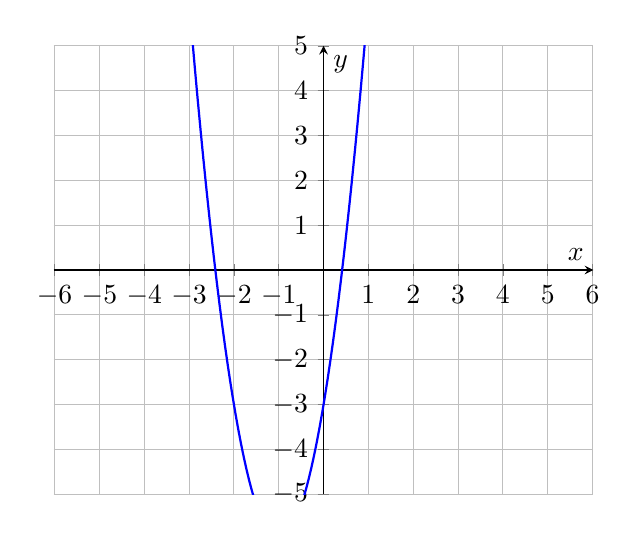
\begin{tikzpicture}
			\begin{axis}[
			axis equal,
			axis x line=middle, 
			axis y line=middle,
			xlabel={$x$},		
			ylabel={$y$},
			xtick={-6,-5,...,6}, 
			ytick={-5,-4,...,5},
			%			minor tick num = 2,
			xmin=-4, xmax=4,
			ymin=-5, ymax=5,
			grid=both,]
			\addplot[domain=-6:6,			samples=200,thick,color=blue,]{3*x^2+6*x-3};	
			\end{axis}
			\end{tikzpicture}
		}
		\solonly{$y=3x^2+6x-3$}
		\end{parts}
		\end{multicols}

 
\end{questions}	

\exnewpage
\subsection{Applicazioni}
\begin{questions}
\question
\exonly{In un decreto  federale del 1889 è stato stipulato che: \textit{La bandiera della Confederazione consiste in una croce bianca verticale posta su di uno sfondo rosso le cui braccia, uguali tra loro, sono di un sesto più lunghe che larghe.} 

Per una festa di decidere di dipingere la croce per terra. Quali saranno le dimensioni della croce se si vogliono usare \SI{204}{\square\metre} di pittura?}

\solonly{Larghezza braccia \SI{6}{\metre}, lunghezza braccia \SI{7}{\metre}}
	
	\question
\exonly{Un giardino a forma rettangolare ha una lunghezza pari al doppio della sua larghezza. Un'aiuola larga \SI{3}{\metre} circonda questo giardino. Calcolare la larghezza del giardino sapendo che la superficie totale (giardino $+$ aiuola) è pari a \SI{360}{\square\metre}. }

\solonly{Larghezza \SI{9}{\metre} }

\question
\exonly{
La'altezza $h(t)$ di un oggetto, lanciato verticalmente da un'altezza di \SI{1}{\metre} con una velocità di \SI{10}{m/s}, dopo $t$ secondi è data da:

$$
h(t)=-\dfrac{1}{2}gt^2+10t+1
$$

dove $g\approx \SI{9.81}{m/s^2}$ .
 }
\begin{parts}
	\part 
	\exonly{Dopo quanti secondi l'oggetto sarà ad un'altezza di \SI{3}{\metre}? (approssimare la risposta ai millisecondi)}
	\solonly{\SI{0.225}{\second} e \SI{1.814}{\second} }
	\part
	\exonly{Dopo quanti secondi l'oggetto sarà ad un'altezza di \SI{10}{\metre}? (approssimare la risposta ai millisecondi)}
	\solonly{Mai }
	\part
	\exonly{Qual'è l'altezza massima che può raggiungere? Dopo quanto tempo la raggiunge? }
	\solonly{Altezza massima \SI{6.097}{\metre} raggiunta dopo \SI{1.019}{\second} }
\end{parts}

\question
\exonly{
Lo standard internazionale del formato carta, l'ISO 216, decreta che il formato A0 è un foglio di carta di \SI{1}{\square\metre} e che i formati successivi (A1, A2, \ldots) si ottengono sempliciemente tagliando a metà la carta sul lato lungo. Per permettere di scalare da un formato all'altro senza compromettere l'aspetto si è deciso che il rapporto tra i due lati di un foglio deve essere costante.
 }

\begin{parts}
	\part
	\exonly{Determinare, a partire dalla definizione, le dimensioni di un foglio di formato A0. }
	\solonly{\SI{0.841}{\metre}$\times$\SI{1.189}{\metre} }
		\part
	\exonly{Determinare, a partire dalla definizione, le dimensioni di un foglio di formato A4. }
	\solonly{\SI{21}{\centi\metre}$\times$\SI{29.7}{\centi\metre} }
\end{parts}


\question
\exonly{
La figura qui sotto mostra la sezione schematizzata di una casa.

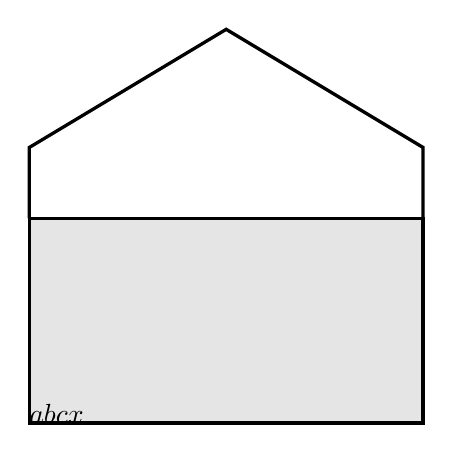
\begin{tikzpicture}
\draw[very thick, fill=gray!20] (0,0) rectangle (5,2.6);
\draw[very thick] (0,2.6) -- (0,3.5) -- (2.5,5) -- (5,3.5) -- (5,2.6);
\dimline[extension start length=-0.3cm,extension end length=-0.3cm] {(0,-0.3)}{(5,-0.3)}{$a$};
\dimline[extension end length=0.3cm,extension start length=0.3cm] {(-0.3,0)}{(-0.3,2.6)}{$b$};
\dimline[extension end length=0.3cm,extension start length=0.3cm] {(-0.3,2.6)}{(-0.3,3.5)}{$c$};
\dimline[extension end length=0,extension start length=0] {(2.5,2.6)}{(2.5,5)}{$x$};
\end{tikzpicture}

}

\begin{parts}
\part
\exonly{Determinare l'altezza $x$ al centro del secondo piano affinché i due piani abbiano la stessa superficie di taglio}
\solonly{\es{$2b-c$}}

\part
\exonly{
Cosa potete constatare?
}
\solonly{La soluzione non dipende da $a$ ma solo da $b$ e $c$.}

\end{parts}

\question
\exonly{Le pagine di un libro d'arte hanno forma rettangolare: larghezza pari a $a$ \si{\centi\metre} e lunghezza pari a 
$b$ \si{\centi\metre}.

Ogni pagina è composta da una zona di testo e da un margine di larghezza constante $x$ \si{\centi\metre}. 

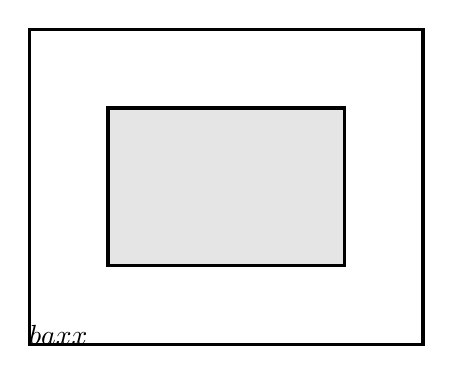
\begin{tikzpicture}
\draw[very thick, fill=gray!20] (1,1) rectangle (4,3);
\draw[very thick] (0,0) rectangle (5,4);
\dimline[color=black,extension start length=-0.3cm, extension end length=-0.3cm] {(0,-0.3)}{(5,-0.3)}{$b$};
\dimline[color=black,extension start length=0.3cm, extension end length=0.3cm] {(-0.3,0)}{(-0.3,4)}{$a$};
\dimline[color=black,extension start length=0, extension end length=0] {(4,2)}{(5,2)}{$x$};
\dimline[extension start length=0, extension end length=0] {(2.5,3)}{(2.5,4)}{$x$};
\end{tikzpicture}

Determinare la misura di tale margine affinché le due zona abbiano la stessa area.
}

\begin{parts}
\part
\exonly{Nel caso di un foglio A4 ($\SI{21}{\centi\metre}\times\SI{29.7}{\centi\metre}$.)
}
\solonly{\SI{3.58}{\centi\metre}}

\part

\exonly{Nel caso generale.}
\solonly{$\dfrac{a+b-\sqrt{a^2+b^2}}{4}$}

\end{parts}

\end{questions}